\documentclass[11pt,letterpaper]{article}
\usepackage[lmargin=1in,rmargin=1in,tmargin=1in,bmargin=1in]{geometry}
\usepackage{../style/homework}
\setbool{quotetype}{true} % True: Side; False: Under
\setbool{hideans}{false} % Student: True; Instructor: False

% -------------------
% Content
% -------------------
\begin{document}

\homework{10: Due 03/04}{I hate these nerds! Just 'cause I'm stupider than them they think they're smarter than me.}{Hubert J. Farnsworth, Futurama}

% Problem 1
\problem{10} Let $f(x)$ be the function given by $f(x)= 4x - 5$. 
	\begin{enumerate}[(a)]
	\item Find a value in the range of $f$. Be sure to justify why the value is in the range. 
	\item Compute $f(-1)$. Is $(-1, -9)$ on the graph of $f$? Explain. 
	\item Is there an $x$ such that $f(x)= 11$? Explain. 
	\item Is $2 \in f^{-1}(0)$? Explain. 
	\item Assuming $f^{-1}$ exists, what is $f(f^{-1}(\sqrt{2}))$ and $f^{-1}(f(\sqrt{2}))$?
	\end{enumerate} \pspace

\sol 
\begin{enumerate}[(a)]
\item The range of $f$ is the set of outputs of $f$. So we can input any value of $x$ in the domain of $f$ into $f$ to obtain an output. For instance, we have\dots
	\[
	f(0)= 4(0) - 5= -5
	\]
Therefore, $-5$ is in the range of $f$. \pspace

\item We have\dots
	\[
	f(-1)= 4(-1) - 5= -4 - 5= -9
	\]
This implies that $(-1, -9)$ is on the graph of $f$. \pspace

\item Suppose there were an $x_0$ such that $f(x_0)= 11$. Then we have\dots
	\[
	\begin{gathered}
	f(x_0)= 11 \\
	4x_0 - 5= 11 \\
	4x_0= 16 \\
	x_0= 4
	\end{gathered}
	\]
Therefore, $x_0= 4$ is a value such that $f(x_0)= 11$. We can confirm this: $f(4)= 4(4) - 5= 16 - 5= 11$. \pspace

\item If $2 \in f^{-1}(0)$, then $f(2)= 0$. But we have $f(2)= 4(2) - 5= 8 - 5= 3 \neq 0$. Therefore, $2 \notin f^{-1}(0)$. \pspace

\item If $f(x)$ has an inverse, then $f \big( f^{-1}(x) \big)= x$ and $f^{-1}\big( f(x) \big)= x$. But then $f(f^{-1}(\sqrt{2}))= \sqrt{2}$ and $f^{-1}(f(\sqrt{2}))= \sqrt{2}$. 
\end{enumerate}



\newpage



% Problem 2
\problem{10} Consider the relation $f$ plotted below. 
	\[
	\fbox{
	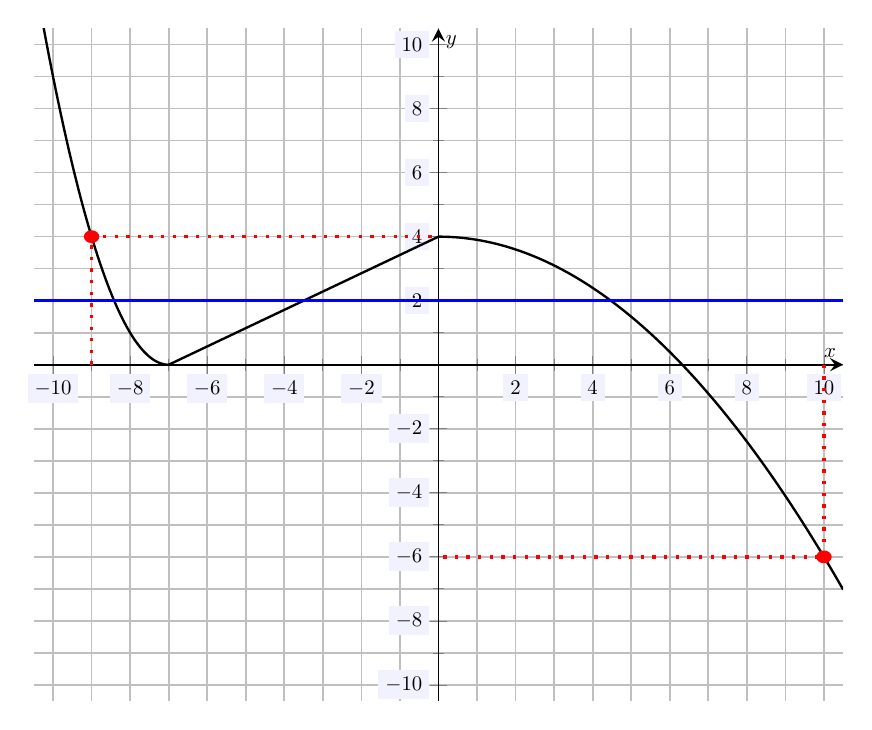
\begin{tikzpicture}[scale=1.5,every node/.style={scale=0.5}]
	\begin{axis}[
	grid=both,
	axis lines=middle,
	ticklabel style={fill=blue!5!white},
	xmin= -10.5, xmax=10.5,
	ymin= -10.5, ymax=10.5,
	xtick={-10,-8,-6,-4,-2,0,2,4,6,8,10},
	ytick={-10,-8,-6,-4,-2,0,2,4,6,8,10},
	minor tick = {-10,-9,...,10},
	xlabel=\(x\),ylabel=\(y\),
	]
	\addplot[line width= 0.02cm,samples=100,domain= -10.5:-7] ({x},{(x + 7)^2}); 
	\addplot[line width= 0.02cm,samples=100,domain= -7:0] ({x},{4/7*x + 4}); 
	\addplot[line width= 0.02cm,samples=100,domain= 0:10.5] ({x},{-x^2/10 + 4}); 
	
	\draw[fill=red,draw=none] (-9,4) circle (0.2);
	\draw[red,dotted,thick] (-9,0) -- (-9,4) -- (0,4);
	
	\draw[fill=red,draw=none] (10,-6) circle (0.2);
	\draw[red,dotted,thick] (10,0) -- (10,-6) -- (0,-6);
	
	\draw[line width=0.03cm,blue] (-10.5,2) -- (10.5,2);
	\end{axis}
	\end{tikzpicture}
	}
	\] 

\begin{enumerate}[(a)]
\item Compute $f(-9)$ and $f(10)$. 
\item Is $f(x)$ a function? Explain. 
\item Does $f(x)$ have an inverse? If so, sketch the inverse. If not, explain why. 
\end{enumerate} \pspace

\sol 
\begin{enumerate}[(a)]
\item Examining the graph of $f(x)$, we see that $f(-9)= 4$ and $f(10)= -6$. \pspace

\item Yes, $f(x)$ is a function because $f(x)$ passes the Vertical Line Test, i.e. every vertical line intersects the graph of $f(x)$ at most once. \pspace

\item The function $f(x)$ does not have an inverse, i.e. $f^{-1}(x)$ does not exist, because not every horizontal line intersects the graph of $f(x)$ at most once. For instance, the horizontal line at $y= 2$ (in blue) intersects the graph of $f(x)$ more than once. 
\end{enumerate}



\newpage



% Problem 3
\problem{10} Showing all your work, verify that $g(x)= \frac{1 - x}{5}$ is the inverse function for $f(x)= 1 - 5x$. Also, compute $g(6)$. What does the value of $g(6)$ tell you about the function $f(x)$? \pspace

\sol If $g(x)$ is the inverse of $f(x)$, then $(f \circ g)(x)= x$ and $(g \circ f)(x)= x$. We have\dots
	\[
	\begin{aligned}
	(f \circ g)(x)&= f \big( g(x) \big)= f \left( \dfrac{1 - x}{5} \right)= 1 - 5 \left( \dfrac{1 - x}{5} \right)= 1 - (1 - x)= x \\[0.3cm]
	(g \circ f)(x)&= g \big( f(x) \big)= g(1 - 5x)= \dfrac{1 - (1 - 5x)}{5}= \dfrac{5x}{5}= x
	\end{aligned}
	\]
Now we have\dots
	\[
	g(6)= \dfrac{1 - 6}{5}= \dfrac{-5}{5}= -1
	\]
From our work above, we know that $g= f^{-1}$. But then $-1= g(6)= f^{-1}(6)$. Recall that $x= f^{-1}(y)$ if and only if $f(x)= y$. Because $f^{-1}(6)= -1$, we must have $f(-1)= 6$. 



\newpage



% Problem 4
\problem{10} A relation $\phi$ is plotted below. 
	\[
	\fbox{
	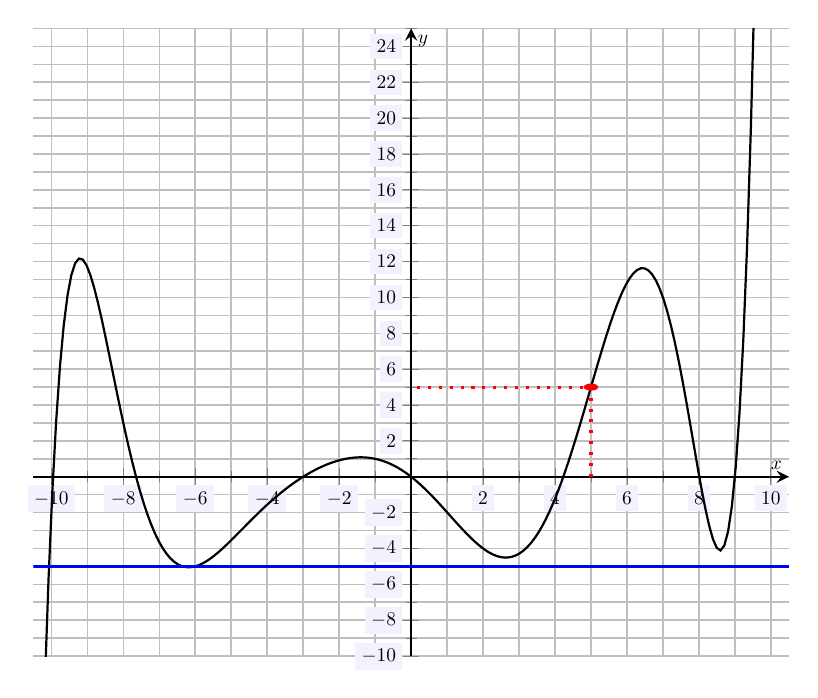
\begin{tikzpicture}[scale=1.4,every node/.style={scale=0.5}]
	\begin{axis}[
	grid=both,
	axis lines=middle,
	ticklabel style={fill=blue!5!white},
	xmin= -10.5, xmax=10.5,
	ymin= -10, ymax=25,
	xtick={-10,-8,-6,-4,-2,0,2,4,6,8,10},
	ytick={-10,-8,...,25},
	minor tick = {-10,-9,...,25},
	xlabel=\(x\),ylabel=\(y\),
	]
	\addplot[line width= 0.02cm,samples=200,domain= -10.5:10.5] ({x},{-1.56755*x - 0.529734*x^2 + 0.0728113*x^3 + 0.039114*x^4 +  0.00344758*x^5 - 0.000794827*x^6 - 0.000120631*x^7 + 0.00000498369*x^8 + 0.000000848123*x^9}); 
	
	\draw[fill=red,draw=none] (5,5) circle (0.2);
	\draw[red,dotted,thick] (5,0) -- (5,5) -- (0,5);
	
	\draw[line width=0.03cm,blue] (-10.5,-5) -- (10.5,-5);
	\end{axis}
	\end{tikzpicture}
	}
	\] 
Using the plot above, answer the following:
	\begin{enumerate}[(a)]
	\item Compute $\phi(5)$.
	\item Find the $y$-intercept for $\phi(x)$. 
	\item Find the $x$-intercepts for $\phi(x)$. 	
	\item As accurately as possible, compute the preimage of $-5$, i.e. $\phi^{-1}(-5)$. 
	\item Explain why (d) implies that $\phi$ does not have an inverse function. 
	\end{enumerate} \pspace

\sol 
\begin{enumerate}[(a)]
\item Examining the graph, we have $\phi(5)= 5$. \pspace

\item The $y$-intercept of $\phi(x)$ is the point where the graph of $\phi(x)$ intersects the $y$-axis. Examining the graph of $\phi(x)$, the $y$-intercept is $(0, 0)$, i.e. $0$. \pspace

\item The $x$-intercept(s) are the point(s) (if there are any) where the graph of $\phi(x)$ intersects the $x$-axis. Examining the plot of $\phi(x)$, we see that the $x$-intercepts of $\phi(x)$ are $x \approx -9.95$, $-7.65$, $-3$, $0$, $4.23$, $8.01$, $9$. \pspace

\item The preimage of $-5$ under $\phi$, i.e. $\phi^{-1}(5)$ are the $x$-value(s) (if they exist) such that $\phi(x)= -5$. Examining the graph of $\phi(x)$ (using the blue line at $y= -5$), we see that $\phi^{-1}(5)= \{ -10.06, -6.35, -6 \}$. \pspace

\item From (d), we know there is more than one possible input such that $\phi(x)= -5$. But then $\phi^{-1}(5)$ cannot be well defined so that $\phi^{-1}$ is not a function. 
\end{enumerate}


\end{document}